\documentclass[a4paper, 12pt]{article}
\usepackage[T2A,T1]{fontenc}
\usepackage[utf8]{inputenc}
\usepackage[english, russian]{babel}
\usepackage{graphicx}
\usepackage[hcentering, bindingoffset = 10mm, right = 15 mm, left = 15 mm, top=20mm, bottom = 20 mm]{geometry}
\usepackage{multirow}
\usepackage{lipsum}
\usepackage{amsmath, amstext}
\usepackage{siunitx}
\usepackage{subcaption}
\usepackage{wrapfig}
\usepackage{adjustbox}
\usepackage{enumerate, indentfirst, float}
\usepackage{capt-of, svg}
\usepackage{icomma}
\usepackage{ctable}

\newenvironment{bottompar}{\par\vspace*{\fill}}{\clearpage}

\begin{document}
	\begin{titlepage}
		
		\newcommand{\HRule}{\rule{\linewidth}{0.5mm}} % Defines a new command for the horizontal lines, change thickness here
		
		\center % Center everything on the page
		
		%----------------------------------------------------------------------------------------
		%	HEADING SECTIONS
		%----------------------------------------------------------------------------------------
		
		\textsc{\LARGE Московский Физико-Технический Институт}\\[1,5cm] % Name of your university/college
		\textsc{\Large Кафедра общей физики}\\[0.5cm] % Major heading such as course name
		\textsc{\large Лабораторная работа \textnumero  3.1.1}\\[0.5cm] % Minor heading such as course title
		
		%----------------------------------------------------------------------------------------
		%	TITLE SECTION
		%----------------------------------------------------------------------------------------
		
		\HRule
		\\[0.4cm]
		{ \huge \bfseries Магнитометр}
		\\[0.2cm] % Title of your document
		\HRule
		\\[1.5cm]
		
		
		
		%----------------------------------------------------------------------------------------
		%	AUTHOR SECTION
		%----------------------------------------------------------------------------------------
		
		\begin{minipage}{0.4\textwidth}
			\begin{flushleft} \large
				\emph{Автор:}\\
				Алексей \textsc{Домрачев} \\
				615 группа
			\end{flushleft}
		\end{minipage}
		~
		\begin{minipage}{0.4\textwidth}
			\begin{flushright} \large
				\emph{Преподаватель:} \\
				\textsc{Дьячков} % Supervisor's Name
			\end{flushright}
		\end{minipage}
		
		\begin{bottompar}
			\begin{center}
				
\includegraphics[width = 80 mm]{logo.jpg}
			\end{center}
			{\large \today}
			
		\end{bottompar}
		\vfill % Fill the rest of the page with whitespace
		
	\end{titlepage}
	
	\paragraph{Цель работы:} определить горизонтальную составляющую магнитного поля Земли и установить количественное соотношение между единицами электрического тока в системе СИ и абсолютной гауссовой системе.
	\paragraph{В работе используются:} магнитометр, осветитель со шкалой, источник питания, вольтметр, электромагнитный переключатель, конденсатор, намагниченный стержень, прибор для определения периода крутильных колебаний, секундомер, рулетка, штангенциркуль
	\section*{Задание 1.}
	\subsection*{Экспериментальная установка}
	\begin{figure}[h]
		\begin{minipage}[h]{0.5\linewidth}
			\center{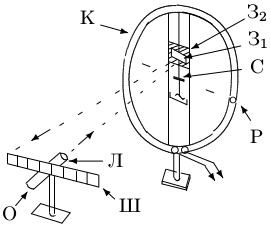
\includegraphics[width=0.5\linewidth]{station.png} \\ a) Схема магнитометра}
		\end{minipage}
		\begin{minipage}[h]{0.5\linewidth}
			\center{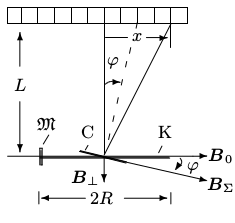
\includegraphics[width=0.5\linewidth]{station2.png} \\ б) Схема измерения угла
				отклонения магнитной стрелки}
		\end{minipage}
		\caption{Устройство магнитометра}
		\label{ris:station}
	\end{figure}
	Магнитометр — прибор для магнитных измерений — это компас, теодолит,веберметр и пр. С помощью магнитометров измеряют намагниченность ферромагнетиков, напряжённость магнитных полей, исследуют магнитные аномалии.\\
	
	\paragraph{Теория. } 
	
	\paragraph{Постановка задачи.} Измерим угол отклонения магнитной стрелки в поле намагниченного стержня и период колебаний этого стержня в поле Земли. По результатам измерений рассчитываем горизонтальную составляющую магнитного поля Земли.
	\paragraph{Выполнение измерений.} В нашей установке магнитную стрелку заменяют сменяют смещения двух световых зайчиков относительно друг друга. Вставляя намагниченный стержень в отверстие P (Рис.~\ref{ris:station}а) измерим смещение подвижного зайчика $x_1=4.7\pm0.05$ см (Рис.~\ref{ris:station}б). Поменяв ориентацию стержня измерим $x_2=4.8\pm0.05$ см. Измерим расстояние от шкалы до зеркала $L=99.0\pm0.1$ см.\\
	Опустим стержень на длинной нити в стеклянный сосуд, и измерим период его колебаний.
	\begin{table}[H]
		\centering
		\caption{Зависимость времени от колебаний}
		\begin{tabular}{c|cccc}
			\toprule
			$t$, с & 63.84 &  56.27 & 56.93 & 54.20    \\
			$N$, колебаний & 4 & 4 & 4 &  4      \\ \midrule
			$T$, с & 15.96 & 14.07 & 14.23 & 13.55 \\ \bottomrule
		\end{tabular}
	\end{table}
	Получаем средний период колебаний $T_\text{ср.} = 14.45\text{ с}$.\\
	Измерим линейные размеры стержня $m = 4.35\text{ г}$, $d=4\text{ мм}$, $l=45\text{ мм}$. Также нам был дан радиус кольца К (Рис.~\ref{ris:station}а) $R=38\text{ см}$.\\ 
	Произведем рассчет момента инерции ферромагнитного стержня: $$J=\dfrac{ml^2}{12}\left[1+3\left(\dfrac{r}{l}\right)^2\right]=7.38 \cdot 10^{-7}\text{ кг/м}^2$$ Теперь рассчитаем магнитное поле: $$B_0=\dfrac{2\pi}{TR}\sqrt{\dfrac{\mu_0JL}{2\pi Rx_1}}=8.91\cdot 10^{-6} \text{ Тл}$$
	
	\section*{Задание 2.}
	\subsection*{Экспериментальная установка}
	\begin{figure}[h]
		\begin{minipage}[h]{0.5\linewidth}
			\center{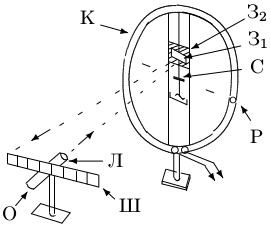
\includegraphics[width=0.5\linewidth]{station.png} \\ a) Схема магнитометра}
		\end{minipage}
		\begin{minipage}[h]{0.5\linewidth}
			\center{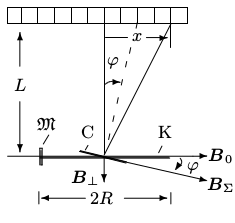
\includegraphics[width=0.5\linewidth]{station2.png} \\ б) Схема измерения угла
				отклонения магнитной стрелки}
		\end{minipage}
		\caption{Устройство магнитометра}
		\label{ris:station}
	\end{figure}
\end{document}